\documentclass[dvipsnames]{beamer}
\mode<presentation>
\usepackage{graphicx}
\usepackage{wasysym}
\usepackage{hyperref}
\definecolor{links}{HTML}{2A1B81}
\hypersetup{colorlinks,linkcolor=,urlcolor=links}
\usepackage{fancyhdr}
\usepackage{multicol}
\usepackage{multirow}
\usepackage{float}
\usepackage{amssymb}
\usepackage{scalerel,stackengine,amsmath}

\usepackage[normalem]{ulem}
\def\Put(#1,#2)#3{\leavevmode\makebox(0,0){\put(#1,#2){#3}}}

\usepackage{tikz}
\usetikzlibrary{arrows,shapes,chains}
\usetikzlibrary{positioning,decorations.pathreplacing}
\usetikzlibrary{fit,shapes.misc}
\usetikzlibrary{decorations.pathreplacing,calc}
\newcommand{\tikzmark}[1]{\tikz[overlay,remember picture] \node (#1) {};}
\tikzset{
	startstop/.style={
		rectangle, 
		rounded corners,
		minimum width=3cm, 
		minimum height=1cm,
		align=center, 
		draw=black, 
		fill=red!30
	},
	process/.style={
		rectangle, 
		minimum width=3cm, 
		minimum height=1cm, 
		align=center, 
		draw=black, 
		fill=blue!30
	},
	decision/.style={
		rectangle, 
		minimum width=3cm, 
		minimum height=1cm, align=center, 
		draw=black, 
		fill=green!30
	},
	arrow/.style={thick,->,>=stealth},
	dec/.style={
		ellipse, 
		align=center, 
		draw=black, 
		fill=green!30
	},
}
\tikzset{cross/.style={cross out, draw, 
		minimum size=2*(#1-\pgflinewidth), 
		inner sep=0pt, outer sep=0pt,color=red},
	decoration={brace},
	tuborg/.style={decorate}}

\tikzset{
	invisible/.style={opacity=0},
	visible on/.style={alt=#1{}{invisible}},
	alt/.code args={<#1>#2#3}{%
		\alt<#1>{\pgfkeysalso{#2}}{\pgfkeysalso{#3}} % \pgfkeysalso doesn't change the path
	},
}  


\usepackage{geometry}
\usepackage{appendixnumberbeamer}

\usepackage{listliketab} %make itemize env behaving like tables !
\usepackage{listings}
\usepackage{setspace}
\usepackage{color}
% General Colors
\definecolor{deepblue}{rgb}{0,0,0.5}
\definecolor{deepred}{rgb}{0.6,0,0}
\definecolor{deepgreen}{rgb}{0,0.5,0}

% Colors for Python
\definecolor{Code}{rgb}{0,0,0}
\definecolor{Decorators}{rgb}{0.5,0.5,0.5}
\definecolor{Numbers}{rgb}{0.5,0,0}
\definecolor{MatchingBrackets}{rgb}{0.25,0.5,0.5}
\definecolor{Keywords}{rgb}{0,0,0.5}
\definecolor{Strings}{rgb}{0,0.63,0}
\definecolor{Comments}{rgb}{0.4,0.4,0.4}
\definecolor{Backquotes}{rgb}{0,0,0}
\definecolor{Classname}{rgb}{0,0,0}
\definecolor{FunctionName}{rgb}{0,0,0}
\definecolor{Operators}{rgb}{0,0,0}
\definecolor{Background}{rgb}{0.93,0.93,0.93}

\definecolor{RWTHbluedark}{RGB}{0,84,159}
\definecolor{RWTHbluelight}{RGB}{142,186,229}
\definecolor{RWTHmagenta}{RGB}{227,0,102}
\definecolor{RWTHmagentalight}{RGB}{249,210,218}
\definecolor{RWTHyellow}{RGB}{255,237,0}
\definecolor{RWTHorange}{RGB}{246,168,0}
\definecolor{RWTHred}{RGB}{204,7,30}
\definecolor{RWTHgreen}{RGB}{87,171,39}
\definecolor{RWTHlila}{RGB}{122,111,172}
\definecolor{RWTHbordeaux}{RGB}{161,16,53}


\newcommand{\self}{\color{CadetBlue}}


\usepackage{epstopdf}
%\usepackage[urlcolor=magenta]{hyperref}
\usepackage{hyperref}
\usepackage{wasysym}
\hypersetup{urlcolor=magenta}


% Default fixed font does not support bold face
% \DeclareFixedFont{\ttb}{T1}{txtt}{bx}{n}{12} % for bold
% \DeclareFixedFont{\ttm}{T1}{txtt}{m}{n}{12}  % for normal


% Python style for highlighting
\newcommand\pythonstyle{\lstset{
showspaces=false,
showtabs=false,
showstringspaces=false,
tabsize=2,
breaklines=true,
% Basic
%basicstyle=\ttfamily\footnotesize\setstretch{1},
basicstyle=\ttfamily\footnotesize\color{black},
backgroundcolor=\color{Background},
language=Python,
% Comments
commentstyle=\color{Comments}\slshape,
% Strings
stringstyle=\color{Strings},
morecomment=[s][\color{Comments}]{"""}{"""},
morecomment=[s][\color{Strings}]{'''}{'''},
morecomment=[l][\color{BurntOrange}]{\@},
% keywords
keywordstyle={\color{Keywords}\bfseries},
keywordstyle=[2]{\color{Magenta}\bfseries},
keywordstyle=[3]{\color{deepred}\bfseries},
keywords={from,class,def,for,while,if,is,in,elif,else,not,and,or,print,break,continue,return,True,False,None,access,as,del,except,exec,finally,global,lambda,pass,print,raise,try,assert},
% additional keywords
keywords=[2]{import, dir, range},
keywords=[3]{__init__},
emph={self},
emphstyle={\self},
%
}}

% C style for highlighting
\newcommand\cstyle{\lstset{
  %language=C,
  showspaces=false,
  showtabs=false,
  showstringspaces=false,
  tabsize=2,
  basicstyle=\ttfamily\scriptsize\color{black},
  backgroundcolor=\color{Background},
  language=C,
  breaklines=true,
  % Comments
  commentstyle=\color{Comments}\slshape,
  % Strings
  stringstyle=\color{Strings},
  %keywordstyle=\color{Keywords}\ttfamily,
  keywordstyle={\color{Keywords}\bfseries},
  keywordstyle=[2]{\color{Magenta}\bfseries},
  keywordstyle=[3]{\color{deepred}\bfseries},
  keywordstyle=[4]{\color{MidnightBlue}\bfseries},
  keywords={for, if, else, return, break, continue, do, double, float, int, char, enum, struct, long, signed, include},
  keywords=[2]{fprintf, sprintf, printf, scanf, sscanf, fscanf},
  keywords=[3]{class_call, class_test, class_alloc, class_calloc,class_define_index},
  keywords=[4]{stderr, stdout, stdin},
  stringstyle=\color{Strings}\ttfamily,
  commentstyle=\color{Comments}\slshape,
  morecomment=[l][\color{magenta}]{\#},
  morecomment=[s][\color{Strings}]{"}{"},
  morecomment=[s][\color{Strings}]{'}{'},
}}

% C style for highlighting
\newcommand\smallcstyle{\lstset{
		%language=C,
		showspaces=false,
		showtabs=false,
		showstringspaces=false,
		tabsize=2,
		basicstyle=\ttfamily\tiny\color{black},
		backgroundcolor=\color{Background},
		language=C,
		breaklines=true,
		% Comments
		commentstyle=\color{Comments}\slshape,
		% Strings
		stringstyle=\color{Strings},
		%keywordstyle=\color{Keywords}\ttfamily,
		keywordstyle={\color{Keywords}\bfseries},
		keywordstyle=[2]{\color{Magenta}\bfseries},
		keywordstyle=[3]{\color{deepred}\bfseries},
		keywordstyle=[4]{\color{MidnightBlue}\bfseries},
		keywords={for, if, else, return, break, continue, do, double, float, int, char, enum, struct, long, signed, include},
		keywords=[2]{fprintf, sprintf, printf, scanf, sscanf, fscanf},
		keywords=[3]{class_call, class_test, class_alloc, class_calloc},
		keywords=[4]{stderr, stdout, stdin},
		stringstyle=\color{Strings}\ttfamily,
		commentstyle=\color{Comments}\slshape,
		morecomment=[l][\color{magenta}]{\#},
		morecomment=[s][\color{Strings}]{"}{"},
		morecomment=[s][\color{Strings}]{'}{'},
}}

% Python environment
\lstnewenvironment{python}[1][]
{
\pythonstyle
\lstset{#1}
}
{}

% Python for external files
\newcommand\pythonexternal[2]{{
\pythonstyle
\lstinputlisting[#1]{#2}}}

% Python for inline
\newcommand\pythoninline[1]{{\pythonstyle\lstinline!#1!}}

% C new environnement
% Python environment
\lstnewenvironment{class}[1][]
{
\cstyle
\lstset{moredelim=[is][\color{red}]{<@}{@>},#1}
}
{}

\lstnewenvironment{smallclass}[1][]
{
	\smallcstyle
	\lstset{moredelim=[is][\color{red}]{<@}{@>},#1}
}
{}
% C for external files
\newcommand\cexternal[2]{{ 
\cstyle
\lstinputlisting[#1]{#2}}}

\newcommand\cinline[1]{{\cstyle\lstinline[]!#1!}}

\newcommand{\equalhat}{\mathrel{\stackon[1.5pt]{=}{\stretchto{%
				\scalerel*[\widthof{=}]{\wedge}{\rule{1ex}{3ex}}}{0.5ex}}}}

% Personal colors
\newcommand{\mygray}{\only{\color{gray}}}
\newcommand{\mywhite}{\only{\color{white}}}
\newcommand{\myblack}{\only{\color{black}}}
\newcommand{\Blue}{\color{Blue}}

%\newcommand{\Red}{\color{BrickRed}}
\newcommand{\Red}{\color{RWTHred}}
\newcommand{\Green}{\color{PineGreen}}
\newcommand{\Purple}{\color{Mulberry}}
\newcommand{\Grey}{\color{gray}}

\renewcommand\mathfamilydefault{\rmdefault}
\usetheme{Warsaw}
\usecolortheme{whale}

\usepackage[T1]{fontenc}
\usepackage[usefilenames,DefaultFeatures={Ligatures=Common}]{plex-otf} %
\usefonttheme{serif}
\setbeamertemplate{itemize item}[circle]
% \renewcommand{\labelitemi}{$\circ$}

% particular color theme
\setbeamercolor{normal text}{fg=RWTHbluedark}
\setbeamercolor{palette primary}{bg=RWTHmagentalight,fg=black}
\setbeamercolor{palette secondary}{bg=RWTHbordeaux,fg=white}
\setbeamercolor{palette tertiary}{bg=RWTHorange,fg=white}
\setbeamercolor{palette quaternary}{bg=RWTHbordeaux,fg=white}
\setbeamercolor{structure}{fg=RWTHbordeaux} % itemize, enumerate, etc
\setbeamercolor{block title}{bg=RWTHbordeaux,fg=white}

\makeatletter
\renewcommand\verbatim@font{\color{black}\normalfont\ttfamily}
\makeatletter

\title[CLASS Basics\hspace{25mm} \insertframenumber/\inserttotalframenumber]{Cosmological Linear Anisotropy Solving System {\scshape (CLASS)}}

\newcommand{\CLASS}{\texttt{class}}
\newcommand{\classy}{\texttt{classy}}
\newcommand{\location}{Les Karellis}
\newcommand{\ecolefromdate}{17}
\newcommand{\ecoletodate}{30}
\author[\ecolefromdate-\ecoletodate.08.2025 \hspace{15mm} M. Mosbech]{Markus R. Mosbech}



\begin{document}


\begin{frame}

\begin{block}{
\begin{center}\Large CLASS\end{center}}
\begin{center}\small Cosmological Linear Anisotropy Solving System \end{center}
\end{block}

\scriptsize

\begin{center}
	% 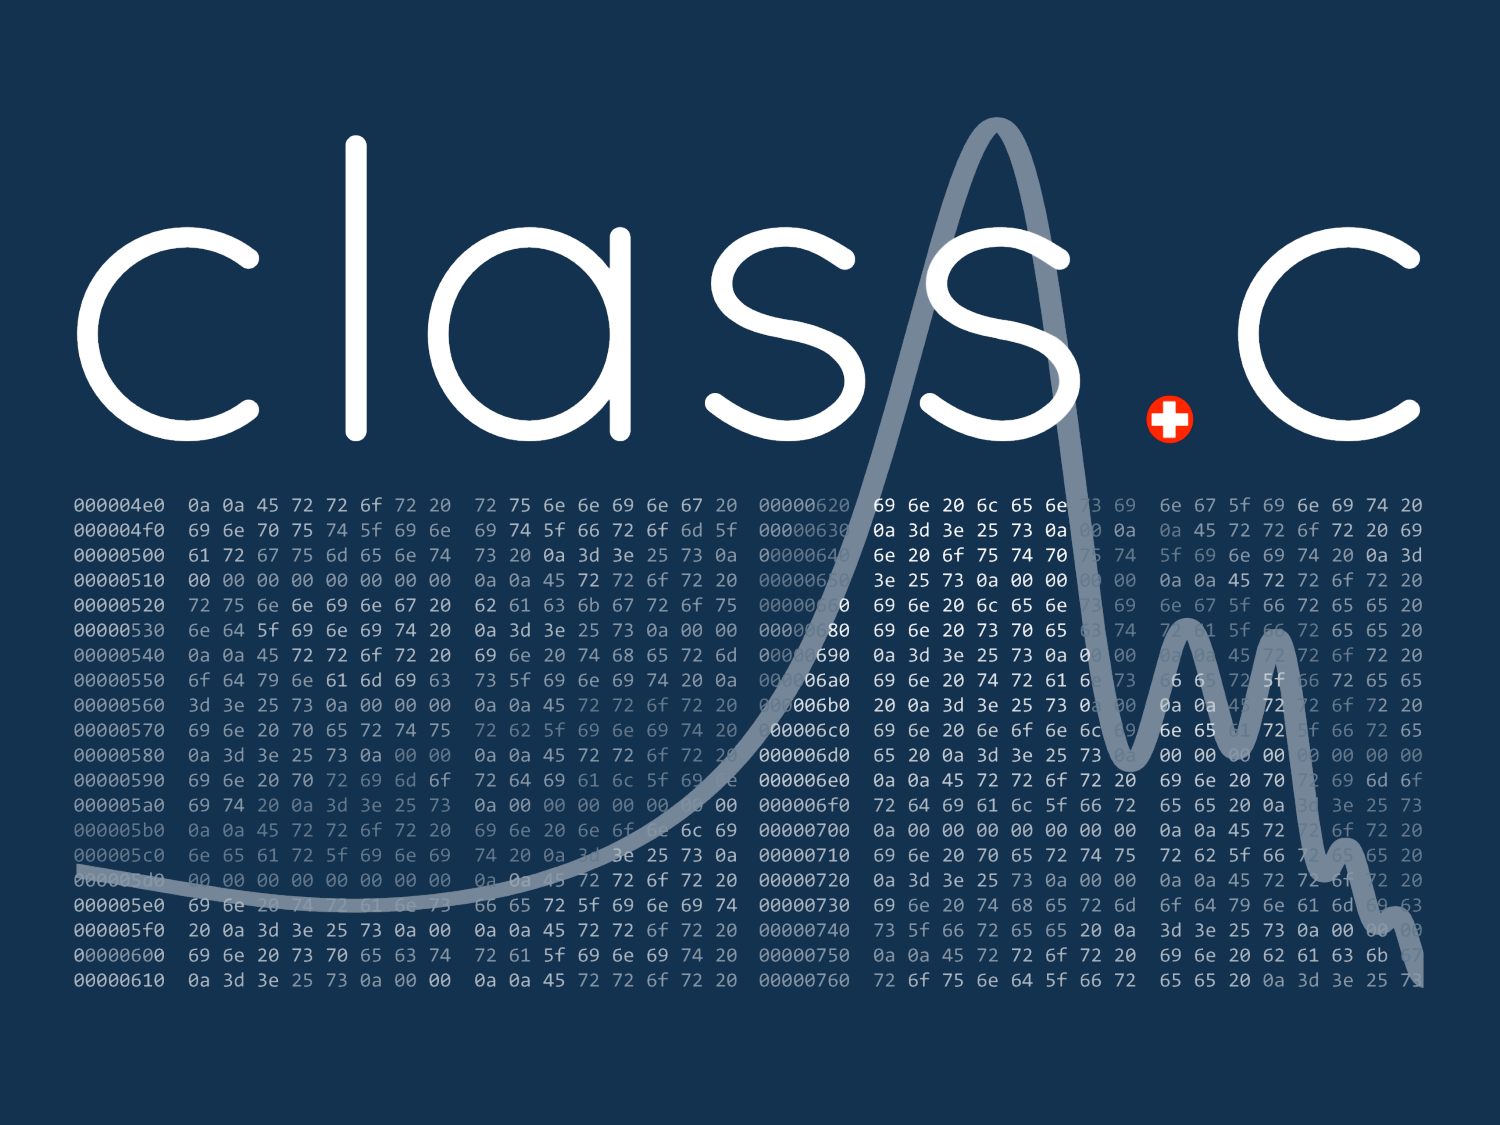
\includegraphics[width=5cm,angle=0]{Logo1b_blue.pdf}\\
	%\framebox{
	Markus Mosbech\\
	Institute for Theoretical Particle Physics and Cosmology, RWTH Aachen University\\
	\mbox{}\\
	\mbox{}\\
	\location, France, \ecolefromdate-\ecoletodate Aug 2025
	%}
	\vfill
	Visit \url{https://lesgourg.github.io/class_public/class.html} for more info!
\end{center}

\end{frame}


\scriptsize

\begin{frame}[fragile]
\frametitle{{\tt \Red class} in \location}

\mbox{}
What to expect in this {\itshape advanced} lecture:
\vspace*{0.5\baselineskip}\mbox{}
\bgroup 
\def\arraystretch{1.15}
\begin{tabular}{lll}
	$\bullet$&Theory:& What is {\Red \tt class} based upon?\\
	$\bullet$&Coding:& Structure of {\Red \tt class}\\
	$\bullet$&Coding:& Essential rules and conventions\\
	$\bullet$&Coding:& Implementing features (C and python)\\
	$\bullet$&Coding:& Using MontePython/Cobaya with {\Red \tt class}
\end{tabular}
\egroup

\mbox{}\\
We will learn {\Red the theory behind \tt class} and the fundamental rules of its {\Red code base}.\\\mbox{}\\
% \begin{center}
\includegraphics[width=8cm,angle=0]{logo-ecole-300.png}\end{center} 

\end{frame}

\begin{frame}[fragile]
\frametitle{{\tt \Red class} Theory}

\begin{enumerate}
	\item Fundamental layout of Einstein-Boltzmann solvers
	\item Essential steps for each module
	\item A few details for each of these steps
\end{enumerate}

\end{frame}

\begin{frame}[fragile]
	\frametitle{Fundamental layout of Einstein-Boltzmann solvers}
	\begin{tikzpicture}[
	start chain=going below,
	every join/.style={arrow,color=black},
	node distance=0.6cm
	]
	\node (bg) [process,on chain,join] {Homogeneous background\\
		$H(a),\rho_i(a),D(a),...$};
	\begin{scope}[start branch]
	\node (th) [process,on chain=going right,join] {Homogeneous thermodynamics\\
		$x_e(z),T_b(z),c_s(z),...$};
	\end{scope}
	\pause
	\draw[tuborg] let
	\p1=(th.north east), \p2=(th.south east) in
	($(\x1+0.5em,\y1)$) -- ($(\x2+0.5em,\y2)$) node[right,midway,xshift=2pt]  {Unify (?)};
	\pause
	\node (pt) [process,on chain,join] {Perturbations\\$\delta_i(k,\tau),\theta_i(k,\tau),...$};
	\begin{scope}[start branch]
	\node (pm) [process,on chain=going right,xshift=4.5em] {Initial condition\\ $P_\mathcal{R}(k)$};
	\end{scope}
	\draw[arrow,color=black] (pm) -- (pt) node[pos=0.4,cross=5pt,sloped] {};
	\draw[arrow,color=red] (pm) -- (pt) node[pos=0.48,sloped,label={[label distance=0.2em,color=red]270:Not required}] {};
	\pause
	\node (obs) [startstop,on chain,join] {Projection\\(LoS/fixed-time)};
	\node (sp) [process,on chain,join] {Correlation functions\\
		$P(k,z),C_\ell$};
	\draw[arrow,color=ForestGreen] (pm) |- (0pt,-70pt) -- (obs.north);
	\draw[arrow,color=black] (th.south) |- (60pt,-25pt)|- (pt.east);
	
	\pause \node [process, below=0mm of bg.north, anchor=north,fill=RWTHbordeaux,text=white] {Background module\\ \texttt{background.c}};
	\pause \node [process, below=0mm of th.north, anchor=north,fill=RWTHbordeaux,text=white] {Thermodynamics module\\ \texttt{thermodynamics.c}};
	\pause \node [process, below=0mm of pt.north, anchor=north,fill=RWTHbordeaux,text=white] {Perturbations module\\ \texttt{perturbations.c}};
	\pause \node [process, below=0mm of pm.north, anchor=north,fill=RWTHbordeaux,text=white] {Primordial module\\ \texttt{primordial.c}};
	\pause \node [startstop, below=0mm of obs.north, anchor=north,fill=RWTHbordeaux,text=white] {Transfer module\\ \texttt{transfer.c}};
	\pause \node [process, below=0mm of sp.north, anchor=north,fill=RWTHbordeaux,text=white] {Harmonic module \& Fourier module\\ \texttt{harmonic.c , fourier.c}};
	\pause \node [process, on chain, join,fill=RWTHbordeaux,text=white] {Lensing module \\ \texttt{lensing.c}};
	\pause \node [process, on chain=going right,fill=RWTHbordeaux,text=white] {Distortions module \\ \texttt{distortions.c}};
	\pause \node [process, on chain=going right,fill=RWTHbordeaux,text=white] {Input \& Output module \\ \texttt{input.c , output.c}};
	\onslide<1->
	\end{tikzpicture}
\end{frame}

\begin{frame}[fragile]
\frametitle{Essential steps in Einstein-Boltzmann solver}
{\centering \Large Let's make a journey through each module!}
\end{frame}

% \section{Modules}

%%%%%%%%% INPUT MODULE

% \subsection{Input Module}

\begin{frame}[fragile]
	\frametitle{Essential steps in Einstein-Boltzmann solver}
	
	{\bf Module 1. Input}\\
	\mbox{}\\
	Read in input files, take care of \textit{shooting}.
	
	\begin{class}
h = 0.7
#H0 = 70
Omega_m = 0.3
#omega_m = 0.14
sigma8=0.8
	\end{class}
	
	\mbox{}\\
	Special care for equivalent/unknown parameters
	
\end{frame}

\begin{frame}[fragile]
	\frametitle{Input management in {\tt \Red class}}
	
	\begin{block}{~~~~~~~~~~~~~~~~~~~~~~~~~~~Terminal~~~~~~~~~~~~~~~~~~~~~~~~~~~~~~~~~~~~~~~~~~~~~~~~~~~~~~~~~~~~~~~~~~Python wrapper}
		\begin{columns}
			\begin{column}{0.5\textwidth} 
				\begin{center}
					file \cinline{xxx.ini}\\
					$\downarrow$\\
					\cinline{input_init(...)}\\
					(parser)\\
					$\downarrow$\\
				\end{center}
			\end{column}
			\begin{column}{0.5\textwidth} 
				\begin{center}
					\mbox{ }\\
					\mbox{ }\\
					\mbox{ }\\
					\cinline{.set(...)}\\
					$\downarrow$\\
				\end{center}
			\end{column}
		\end{columns}
		\vspace{-0.3cm}
		\begin{center}
			\cinline{struct file_content fc;} (all parameter names/values stored as arrays of strings)\\
			$\downarrow$\\
			\cinline{input_read_from_file(...)}\\
			$\downarrow$\\
			\cinline{input_read_parameters(...)}\\
			(assign all default values + interprete input + update some parameters)\\
			$\downarrow$\\
			Only {\it relevant} parameters get stored in the structures of each module
		\end{center}
	\end{block}
\end{frame}

\begin{frame}[fragile]
	\frametitle{Input management in {\tt \Red class}}
	
	For indirect parameters, use {\Red shooting method}\\
	\mbox{ }\\
	
	Repeated calls of \cinline{input_read_parameters(...)}, {\Red \texttt{class}} executions, from \cinline{input_read_from_file(...)} until shooting target is met.\\
	\mbox{ }\\
	
	\pause
	Example:\\
	How would you code the input parameter $\theta_s$?\\
	Use approximate formula $\to$ inflexible, inaccurate\\
	\mbox{ }\\
	
	\pause
	Try out a few values and narrow down (Example: User wants $100 \theta_s = 1.04325$)
	\begin{center}
		\begin{tabular}{|l|r|}
			$h$ & $100 \theta_s$ \\
			\hline
			{\Green 0}.7 & {\Green 1.0}522492086422521 \\
			{\Green 0.6}5 & {\Green 1.0}270326366580724 \\
			{\Green 0.68}215616173 & {\Green 1.043}7999980620178 \\
			{\Green 0.681}10138476 & {\Green 1.0432}819283581667 \\
			{\Green 0.681036}37942 & {\Green 1.0432}499363679562 \\ 
			{\Green 0.6810365}0871 & {\Green 1.0432}499921072458 \\
			{\Green 0.681036527}01 & {\Green 1.04325000}79710365 \\
			 ... & ...
		\end{tabular}
	\end{center}
	
	\pause
	\mbox{}\\
	In practice, use more sophisticated Ridder's method / Newton's method
\end{frame}

\begin{frame}[fragile]
	\frametitle{Input management in {\tt \Red class}}
	
	For {\Red shooting} parameters, establish mapping between {\it target parameter}, {\it unknown parameter} and {\it level}. Currently:
	\begin{center}
		\begin{tabular}{|c|c|c|}
			\hline
			target parameter & unknown parameter & level\\
			\hline
			$100 \times \theta_s$ & $h$ & thermodynamics \\
			$\Omega_\mathrm{dcdm}$ & $\rho^\mathrm{ini}_\mathrm{dcdm}$ & background \\ \sout{$\sigma_8$} & \sout{$A_s$} & \sout{spectra} \\
			... & ... & ...\\
			\hline
		\end{tabular}
	\end{center}
	... plus a few others (alternative parametrizations of decaying CDM, quintessence parameters).\\
	\mbox{}\\
	This is what is used e.g. in models of early dark energy!\\
	
	\vspace{1cm}
	
	If you need to add such parameters: see how it is done e.g. for \cinline{100*theta_s} and replicate the structure!\\
	\mbox{}\\
	{\color{purple}Special exception} $\tau_\mathrm{reio} \leftrightarrow z_\mathrm{reio}$ only concerns reionization and is done independently in \texttt{thermodynamics.c}
	\mbox{}\\
	{\Red New Special exception:} $\sigma_8 \leftrightarrow A_s$ can be very simply analytically re-scaled (multiplicative property), therefore done independently in \texttt{input.c}
\end{frame}




\begin{frame}[fragile]
	\frametitle{Input management in {\tt \Red class}}
	
	{\Red Budget equation:}
	$$
	\sum_X \Omega_X = 1 + \Omega_k
	$$
	To avoid over-constraining the input, one of the last three (\cinline{Omega_Lambda}, \cinline{Omega_fld}, \cinline{Omega_scf}) must be left unspecified and  {\tt \Red class} will assign it using budget equation.\\
	{\tiny Possibly more advanced in the future} 
	\begin{itemize}
		\item default: \cinline{Omega_Lambda} is automatically adjusted
		\item if you pass \cinline{Omega_Lambda},  \cinline{Omega_fld}  is automatically adjusted
		\item if you pass \cinline{Omega_Lambda} and \cinline{Omega_fld}: \cinline{Omega_scf} is automatically adjusted (if you allow, by setting to -1)
	\end{itemize}
	This allows whatever combination.\\
	E.g. to get $\Lambda$ plus a DE fluid: \\
	\cinline{Omega_Lambda=0.2}, \cinline{Omega_scf=0}~~~~or~~~~\cinline{Omega_fld=0.3}, \cinline{Omega_scf=0}
	
	\mbox{}\\
	Helpful output by setting background verbose \texttt{\textgreater= 2}
\end{frame}

%%%%%%%%%%%%%%%%%%%%%%%%%%%%%%%%%%%%%% Background

% \subsection{Background Module}


\begin{frame}[fragile]
\frametitle{Essential steps in Einstein-Boltzmann solver}

{\bf Module 2. Background}\\
\mbox{}\\
Get all background quantities as function of a scale factor $a$.


% ~~~~~~~~~~~~~~~~~~~~~~~~~~~~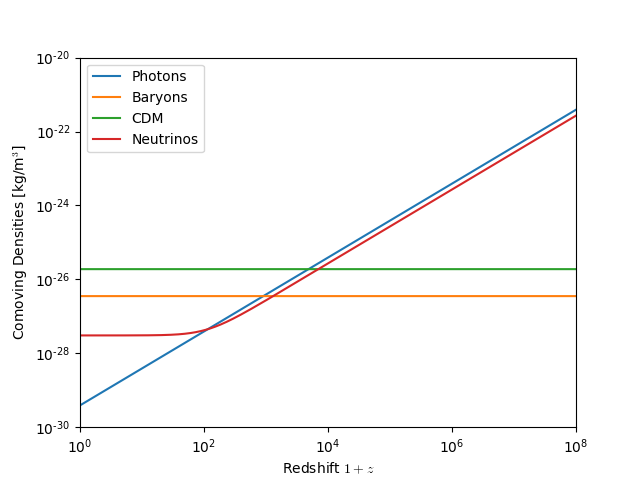
\includegraphics[width=5cm,angle=0]{figs/background.png}

\mbox{}\\
This also gives mapping $a \leftrightarrow z \leftrightarrow t \leftrightarrow \mathrm{conf. time}$\\

\end{frame}

%%
%$$
%H^2 =  \frac{8 \pi G}{3} \sum_X \rho_X(a)    - \frac{K}{a^2}
%$$

\begin{frame}[fragile]
\frametitle{Details of the steps in Einstein-Boltzmann solvers}

Let's formalize problem!\\

\vspace{0.2cm}

Three types of parameters:
\begin{itemize}
	\item {\Green $\{A\} $} are analytical functions of scale factor and {\Green $\{B\}$} quantities.
	%\pause
	\item {\Green $\{B\} $} need to be integrated over, and are used to compute {\Green $\{A\}$}
	%\pause
	\item {\Green $\{C\} $} also need to be integrated over, but are not used to compute {\Green $\{A\}$}.
\end{itemize}


%\pause
\vspace{0.2cm}
\only<2>{
$\Lambda$CDM and many simple extensions:
\begin{itemize}
	\item {\Green $\{A\}$} $= \{\rho_i(a), p_i(a), H(a), ..., \}$ with e.g. $H(a) = \left( \sum_X \rho_x(a) - \frac{K}{a^2} \right)^{1/2}$
	\item {\Green $\{B\}$} $= \{\}$ (eliminated since {\tt \color{black} v3.0})
	\item {\Green $\{C\}$} $= \{t, \tau, r_s, D, f\}$ with e.g. $\frac{dt}{da} = 1/H(a)$, $\frac{d r_s}{d a} = c_s(a)/(a \cdot H(a))$
\end{itemize}}

% \pause
% \vspace{0.2cm}
\only<3>{
Example of DE/DM/DR fluid: 
\begin{itemize}
	\item {\Green $\{A\}$} $= \{\rho_i(a), p_i(a), H(a), ..., {\Red w_{\rm fld}(a)}\}$
	\item {\Green $\{B\}$} $= \{{\Red \rho_{\rm fld}}\}$ with $\frac{d \rho_{\rm fld}}{da} = -3  (1+w_{\rm fld}(a)) \rho_{\rm fld}$
\end{itemize}}

% \pause
% \vspace{0.2cm}
\only<4>{
Exemple of extended cosmology with quintessence $\phi$: 
\begin{itemize}
	\item {\Green $\{A\}$} $ = \{\rho_i, p_i, H, ..., {\Red V(\phi), \rho_\phi(\phi, \phi')} \}$ with e.g. $\rho_\phi(\phi, \phi') = \frac{1}{2} (\phi^\prime)^2 + V(\phi)$
	\item {\Green $\{B\}$} $ = \{{\Red \phi, \phi^\prime}\}$ with $\frac{d \phi}{d a} = \phi'/[aH(a)]$, $\frac{d \phi'}{da} = -2 \phi' - a V(\phi)/H(a)$
\end{itemize}}

% \pause
% \vspace{0.2cm}
\only<5>{
Also Cold Dark Matter decaying into Dark Radiation...
\begin{itemize}
	\item {\Green $\{A\}$} $= \{\rho_i, p_i, H, ... \}$
	\item {\Green $\{B\}$} $= \{{\Red \rho_{\rm dcdm}, {\Red \rho_{\rm dr}}}\}$ with $\frac{d \rho_{\rm dcdm}}{d a} = -3 \rho_{\rm dcdm} - \Gamma\!(a)/H(a) \cdot \rho_{\rm dcdm}$
\end{itemize}}

\end{frame}


\begin{frame}[fragile]
	\frametitle{Details of the steps in Einstein-Boltzmann solvers}

	Small details:
	\begin{itemize}
		\item Quantities as $D_A(z), D_L(z), r_s, t_\mathrm{age}$ can be derived after all A,B,C are computed
		\item Takes care of NCDM integration of phase-space distribution
		\item Useful checks \& output
		\item $\to$ Budget equation output at verbosity level 2
	\end{itemize}
	
\end{frame}

%%%%%%%%%%%%%%%%%%% Thermodynamics

% \subsection{Thermodynamics}

\begin{frame}[fragile]
\frametitle{Essential steps in Einstein-Boltzmann solver}

{\bf Module 3. Thermodynamics}\\
\mbox{}\\
Get all thermodynamics quantities as function of a time variable ({\tt \Red class} $\rightarrow$ redshift $z$) after integrating differential equations like recombination equations:
$$
\frac{d x_e}{dz} , \frac{d T_b}{dz}= {\rm excitation}, {\rm ionization}, {\rm heating}, ... 
$$
\vspace{-0.5cm}\\
% ~~~~~~~~~~~~~~~~~~~~~~~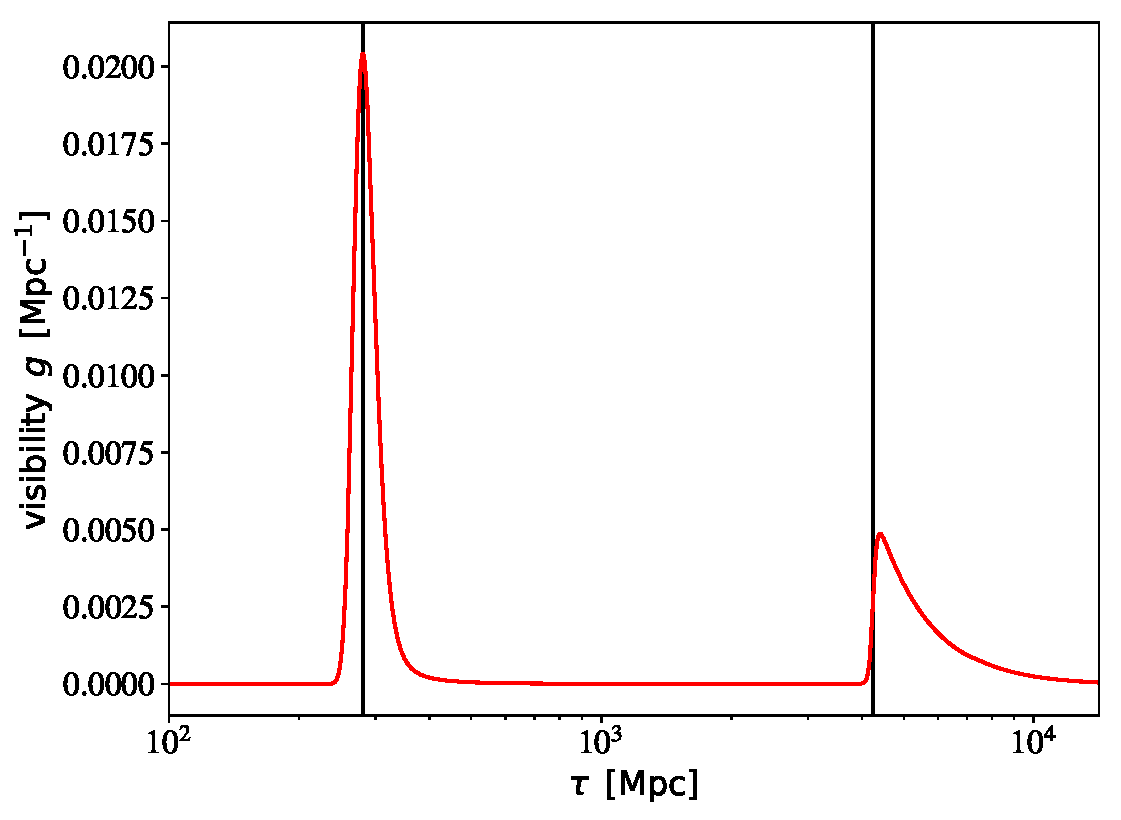
\includegraphics[width=5cm,angle=0]{output_plots/thermo.pdf}\\
Then $x_e(z) \rightarrow \kappa'(z)$ (Thomson scattering rate)\\
~~~~~~~~~~~~~~~$\rightarrow \kappa(z)$ (Optical depth)\\
~~~~~~~~~~~~~~~$\rightarrow \exp(-\kappa(z))$ (factor for Integrated Sachs-Wolfe effect)\\
~~~~~~~~~~~~~~~$\rightarrow g(z)$ (visibility function for Sachs-Wolfe effect)\\
~~~~~~~~~~~~~~~$\rightarrow g'(z)$ (factor for Doppler effect)\\

\end{frame}


\begin{frame}[fragile]
	\frametitle{Details of the steps in Einstein-Boltzmann solvers}
	
	Simplest model of {\Red recombination} is the {\Red Saha equation}.\\ \mbox{}\\ 
	
	It is well known that a non-relativistic ($T \ll m$) species in thermal equilibrium obeys
	\begin{equation}
		n(\mu,T) \approx g e^{\mu/T} \left(\frac{m T}{2 \pi}\right)^{3/2} e^{-m/T}
	\end{equation}
	
	Thus we find using {\Red complete thermal equilibrium} with $\mu_\mathrm{ionized} + \mu_e = \mu_\mathrm{rec}$ that
	\begin{equation*}
		\frac{n_e n_\mathrm{ionized}}{n_\mathrm{rec}} \approx {\Red \left(\frac{m_e T}{2\pi}\right)^{3/2} e^{-E_\mathrm{bind}/T}} \times \underbrace{\left[ e^{\mu_\mathrm{ionized} + \mu_e - \mu_\mathrm{rec}} \left(\frac{g_e g_\mathrm{ionized}}{g_\mathrm{rec}}\right) \left(\frac{m_\mathrm{ionized}}{m_\mathrm{rec}}\right)^{3/2}\right]}_{\approx 1}
	\end{equation*}
	\vspace*{-2\baselineskip}
	This gives
	\begin{equation}
		\frac{x_e^2}{1-x_e} \approx \left(\frac{1.1 \cdot 10^{-10}}{n_\mathrm{H,0} /T_\mathrm{cmb,0}^3}\right) \left(\frac{\mathrm{eV}}{T}\right)^{3/2} {\Red \exp(39.9 - 13.6 \frac{\mathrm{eV}}{T})}
	\end{equation}
	and thus recombination at $T \approx \frac{13.6\mathrm{eV}}{39.9} \approx 0.34\mathrm{eV}$ $\to z \approx 1400$. \pause This is of course wrong...\\ \pause
	{\Red recombination is a non-equilibrium process}
\end{frame}


\begin{frame}[fragile]
\frametitle{Details of the steps in Einstein-Boltzmann solvers}

The {\Red effective multi-level atom} is the basis for recombination codes.\\ \mbox{}\\

1s 2s 2p 3s 3p 3d ... ionized $\to$ 1s 2s 2p ionized \\ \mbox{}\\

\pause
Reason: Intermediate transitions (4p$\to$3s) or (3s$\to$2p) are comparatively instant. Why? Direct transition $2s \to 1s$ is forbidden, and $2p \to 1s$ is immediately reversed by $1s \to 2p$. The medium is {\Red optically thick} during recombination.\\ \mbox{}\\

\pause
Instead, focus on $2p \to 1s$ with subsequent redshifting of photon to escape reabsorption (slow) or $2s \to 1s$ with two-photon decay (slow). \\ \mbox{}\\

{\Red Peeble's equation}
\begin{equation}
	\dot{x_e} \approx f_\mathrm{photo-ion}(T) x_\mathrm{rec}-f_\mathrm{rec}(T) x_e x_\mathrm{ionized} 
\end{equation}
Solved numerically, basis of {\Red recfast}
\end{frame}



\begin{frame}[fragile]
	\frametitle{Details of the steps in Einstein-Boltzmann solvers}
	
	{\Red recfast} only resolves $2s \approx 2p$\\ \mbox{}\\
	\pause
	Improvement: {\Red HyRec} with EMLA resolves $2s,2p$. Even more, can do $2s,2p,3s,...$ with \textit{effective} rates.\\ \mbox{}\\
	
	Fullest code to date: {\Red CosmoRec} does full numerical computation (iteratively). Comparatively slow, but highest achievable accuracy\\ \mbox{}\\
	
	\pause
	Further complication: Helium (higher elements don't contribute)\\
	% ~~~~~~~~~~~~~~~~~~~~~~~\includegraphics[width=5cm,angle=0]{output_plots/thermo2.pdf}\\
\end{frame}


\begin{frame}[fragile]
\frametitle{Details of the steps in Einstein-Boltzmann solvers}

User can choose to model approximate recombination and get $x_e(z)$, $T_b(z)$ from:
\begin{itemize}
\item {\Green RECFAST} (Wong, Moss \& Scott 2008)
\item {\Green HyRec-2} (Y. Ali-Ha\"{\i}moud, N. Lee)
\item Possibly soon? {\Green CosmoRec} (J. Chluba)
\end{itemize}

\pause
\vspace{0.2cm}

Recombination needs one more cosmological parameter: the {\Red primordial Helium fraction} $Y_\mathrm{He}$.
\begin{itemize}
\item Fix it (\cinline{Y_He = 0.25})
\item Get it from BBN (\cinline{Y_He = BBN}). {\tt \Red class} has interpolation table pre-pcomputed with a {\Red BBN code} ({\Green Parthenope}), for each given value of $N_\mathrm{eff}$, $\omega_b$ (assumes $\mu_{\nu_e}=0$, easy to generalize).
\item BBN interpolation table located in separate directory (in \cinline{external/bbn/sBBN_2017.dat}, update inbound)
\end{itemize}


\mbox{}\\

\end{frame}


\begin{frame}[fragile]
	\frametitle{Details of the steps in Einstein-Boltzmann solvers}
	
	For reionization:
	\begin{itemize}
		\item tanh with complicated argument (like {\tt \Red CAMB})
		\item multi-tanh
		\item half tanh
		\item from file (either linear or tanh)
	\end{itemize}
	
	\pause 
	\vspace{0.2cm}
	Mini-shooting to find $z_\mathrm{reio}$ for given $\tau_\mathrm{reio} = \kappa_\mathrm{reio}$. 
	
	Optical depth $\kappa(z)$ = inverse number of expected interactions  $\Rightarrow \kappa'(z) = a n_H x_e \sigma_T$\\
	% \includegraphics[width=5cm,angle=0]{output_plots/thermo_kappa.pdf}\includegraphics[width=5cm,angle=0]{output_plots/thermo_kappa_integrated.pdf}\\
\end{frame}


\begin{frame}[fragile]
	\frametitle{Details of the steps in Einstein-Boltzmann solvers}

	We also include
	\begin{itemize}
		\item Energy injection (increases ionization, heats $T_b$)

		This can cause changes in scattering $\kappa(z)$ and thus be observable with CMB
		\item Time-dependent fundamental constants $\to$ Causes shift in recombination due to fundamental dependencies such as $E_\mathrm{binding} = \frac{1}{2}\alpha^2 m_e= 13.6\mathrm{eV} \left(137 \alpha\right)^2 \left(\frac{m_e}{511\mathrm{keV}}\right)$
		\\
		We remind ourselves $1+z_\mathrm{rec} = T_\mathrm{rec}/T_\mathrm{cmb} \approx \frac{E_\mathrm{binding}}{12.57\mathrm{meV}}$
		\item Computation of useful quantities $z_\mathrm{rec}, z_\mathrm{drag}, z_*, D_A(z_\mathrm{rec}), r_s(z_\mathrm{drag}), ...$
	\end{itemize}
\end{frame}





\end{document}
